% THIS IS SIGPROC-SP.TEX - VERSION 3.1
% WORKS WITH V3.2SP OF ACM_PROC_ARTICLE-SP.CLS
% APRIL 2009
%
% It is an example file showing how to use the 'acm_proc_article-sp.cls' V3.2SP
% LaTeX2e document class file for Conference Proceedings submissions.
% ----------------------------------------------------------------------------------------------------------------
% This .tex file (and associated .cls V3.2SP) *DOES NOT* produce:
%       1) The Permission Statement
%       2) The Conference (location) Info information
%       3) The Copyright Line with ACM data
%       4) Page numbering
% ---------------------------------------------------------------------------------------------------------------
% It is an example which *does* use the .bib file (from which the .bbl file
% is produced).
% REMEMBER HOWEVER: After having produced the .bbl file,
% and prior to final submission,
% you need to 'insert'  your .bbl file into your source .tex file so as to provide
% ONE 'self-contained' source file.
%
% Questions regarding SIGS should be sent to
% Adrienne Griscti ---> griscti@acm.org
%
% Questions/suggestions regarding the guidelines, .tex and .cls files, etc. to
% Gerald Murray ---> murray@hq.acm.org
%
% For tracking purposes - this is V3.1SP - APRIL 2009

\documentclass{acm_proc_article-sp}

\usepackage{url}
\usepackage{algorithmic}
\usepackage{algorithm}
\usepackage{listings}
% \usepackage{draftwatermark}
% \SetWatermarkText{DRAFT}
% \SetWatermarkScale{5}
% "define" Scala
\lstdefinelanguage{scala}{morekeywords={class,object,trait,extends,with,new,if,while,for,def,val,var,this},
otherkeywords={->,=>},
sensitive=true,
morecomment=[l]{//},
morecomment=[s]{/*}{*/},
morestring=[b]"}
% Default settings for code listings
\lstset{frame=tb,language=scala,aboveskip=3mm,belowskip=3mm,showstringspaces=false,columns=flexible,basicstyle={\small\ttfamily}}

\begin{document}

\title{Rethinking Data-Intensive Science Using \linebreak Scalable Analytics Systems}
%
% You need the command \numberofauthors to handle the 'placement
% and alignment' of the authors beneath the title.
%
% For aesthetic reasons, we recommend 'three authors at a time'
% i.e. three 'name/affiliation blocks' be placed beneath the title.
%
% NOTE: You are NOT restricted in how many 'rows' of
% "name/affiliations" may appear. We just ask that you restrict
% the number of 'columns' to three.
%
% Because of the available 'opening page real-estate'
% we ask you to refrain from putting more than six authors
% (two rows with three columns) beneath the article title.
% More than six makes the first-page appear very cluttered indeed.
%
% Use the \alignauthor commands to handle the names
% and affiliations for an 'aesthetic maximum' of six authors.
% Add names, affiliations, addresses for
% the seventh etc. author(s) as the argument for the
% \additionalauthors command.
% These 'additional authors' will be output/set for you
% without further effort on your part as the last section in
% the body of your article BEFORE References or any Appendices.

%  in this sample file, there are a *total*
% of EIGHT authors. SIX appear on the 'first-page' (for formatting
% reasons) and the remaining two appear in the \additionalauthors section.
%
\author{}
% You can go ahead and credit any number of authors here,
% e.g. one 'row of three' or two rows (consisting of one row of three
% and a second row of one, two or three).
%
% The command \alignauthor (no curly braces needed) should
% precede each author name, affiliation/snail-mail address and
% e-mail address. Additionally, tag each line of
% affiliation/address with \affaddr, and tag the
% e-mail address with \email.
%
% 1st. author% There's nothing stopping you putting the seventh, eighth, etc.
% author on the opening page (as the 'third row') but we ask,
% for aesthetic reasons that you place these 'additional authors'
% in the \additional authors block, viz.

% Just remember to make sure that the TOTAL number of authors
% is the number that will appear on the first page PLUS the
% number that will appear in the \additionalauthors section.

\maketitle

\begin{abstract}
Revolutions in data acquisition are drastically changing how scientists make discoveries. ``Next
generation'' sequencing technologies are allowing scientists to collect exponentially more data at a lower
cost. Similar trends impact many fields which rely on imaging, such as astronomy and neuroscience.
Early attempts to use MapReduce systems to accelerate the processing of these datasets have been
limited through the use of legacy data formats that limit horizontal scalability.

In this paper, we demonstrate an example genomics pipeline that leverages open-source MapReduce
and columnar storage techniques to achieve a $22-130\times$ speedup over traditional genomics
systems, at half the cost. From building this system, we were able to distill a set of principles for
implementing scientific analyses efficiently using commodity ``big data'' systems. To demonstrate the
generality of our architecture, we then achieve an average of $5.8\times$ improvement over the state-of-the-art MPI-based system for an astronomy task at different scales.
\end{abstract}

% A category with the (minimum) three required fields
\category{L.4.1}{Applied Computing}{Life and medical sciences}[Computational biology]
\category{H.1.3.2}{Information Systems}{Data management systems}[Database management
system engines, parallel and distributed DBMSs]
\category{E.3.2}{Software and its Engineering}{Software creation and management}[Software
Development Process Management]

\terms{Design}

\keywords{Analytics, MapReduce, Genomics, Scientific Computing}

\section{Introduction}
\label{sec:introduction}

Major improvements in scientific data acquisition techniques have increased scientific data storage and
processing \linebreak needs~\cite{schadt10, cunningham14}. In fields like
neuroscience~\cite{freeman14} and \linebreak genomics~\cite{stein10}, particle physics, and astronomy
scientists routinely perform analysis that use terabytes~(TB) to \linebreak petabytes~(PB) of data.
While traditional scientific computing platforms are optimized for fast linear algebra, many emerging
domains make heavy use of statistical learning techniques and user defined functions~(UDFs) on top of
semistructured data. This move towards statistical techniques has been driven by the increase in the
amount of data available to scientists, as well as the rise of statistical systems that are accessible to
non-experts, such as \texttt{Scikit-learn}~\cite{pedregosa11} and \texttt{MLI}~\cite{sparks13}. At the
same time, commercial needs~(driven by a similar but less dramatic increase in available data) have
led to the development of horizontally-scalable analytics systems like MapReduce~\cite{dean04, dean08}
and Spark~\cite{zaharia10}.

Since the amount of scientific data being generated is growing so quickly, we cannot afford to be
saddled by legacy software and formats which are incompatible with horizontal scalability. New scientific
projects such as the 100K for UK, which aims to sequence the genomes of 100,000 individuals in the
United Kingdom~\cite{uk100k} will generate three to four \emph{orders of magnitude} more data than
prior projects like the 1000 Genomes Project~\cite{siva08}. These projects use the current ``best
practice'' genomic variant calling pipeline~\cite{auwera13}, which takes approximately 120 hours to
process a single, high-quality human genome using a single, beefy node~\cite{talwalkar14}. To address
these challenges, scientists have started to apply computer systems techniques such as
MapReduce~\cite{mckenna10, schatz09, langmead09} and columnar storage~\cite{fritz11} to custom
scientific compute/storage systems. While these systems have improved the analysis cost and
performance, current implementations incur significant overheads imposed by the legacy formats and
codebases that they are built from.

In this paper, we demonstrate a system built using Apache Avro, Parquet, and Spark~\cite{avro, parquet,
zaharia10}, that achieves a 50$\times$ increase in throughput over the current best practice pipeline
for processing genomic data, while reducing the analysis cost by 50\%. In the process of creating this
system, we developed a ``narrow waisted'' layering model for building similar scientific analysis systems.
This narrow waisted stack is inspired by the OSI model for networked systems~\cite{zimmermann80}.
However, in our stack model, the data schema is the narrow waist that separates data processing from
data storage. Our stack solves the following three problems that are common across current scientific
analysis systems:

\begin{enumerate}
\item Current scientific systems improve the performance of common patterns by changing the data
model (often by requiring data to be stored in a coordinate-sorted order).
\item Legacy data formats were not designed with horizontal scalability in mind.
\item The system must be able to efficiently access shared metadata, and to slice datasets for running
targeted analyses.
\end{enumerate}

We solve these problems by:

\begin{enumerate}
\item We make a schema the ``narrow waist'' of our stack and enforce data independence. We then
devise algorithms for making common scientific processing patterns~(e.g., coordinate-space joins,
see~\S\ref{sec:coordinate-system-joins}) fast.
\item To improve horizontal scalability, we use Parquet, a modern parallel columnar store based off of
Dremel~\cite{melnik10} to push computation to the data.
\item We use a denormalized schema to achieve O(1), parallel access to metadata.
\end{enumerate}

Our solution manifests in the design of the stack model for composing scientific systems which is
described in Figure~\ref{fig:stack-model}. We demonstrate the generality of this model by using it to
implement a system for processing astronomy images, which achieves an average of $5.8\times$ performance
improvement over a state-of-the-art Message Passing Interface~(MPI) based pipeline at various scales.

\begin{figure}[h]
\begin{center}
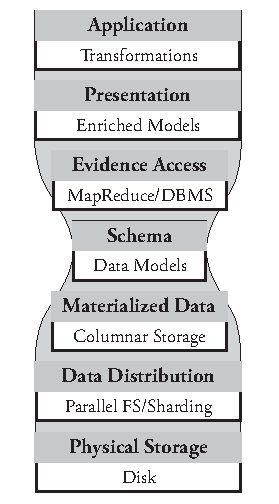
\includegraphics[width=0.6\linewidth]{stack-model.pdf}
\end{center}
\caption{A Stack Model for Scientific Computing}
\label{fig:stack-model}
\end{figure}

While the abstraction inversion used in genomics to accelerate common access patterns is undesirable
because it violates data independence, in this paper, we also find that it sacrifices performance and
accuracy. The current Sequence/Binary Alignment and Map~(SAM/BAM~\cite{li09}) formats for storing
genomic alignments apply constraints about record ordering to enable specific computing patterns. Our
implementation~(described in~\S\ref{sec:genomics-pipeline}) identifies errors in two current genomics
processing stages that occur \emph{because} of the sorted access invariant. Our implementations of
these stages do not make use of sort order, and achieve higher performance \emph{while} eliminating
these errors.

We have made all of the software~(source code and executables) described in this paper available free
of charge under the permissive Apache 2 open-source license.

\section{Background}
\label{sec:background}

Our work exists at the intersection of computational science, data management, and processing
systems. As such, our architectural approach is informed by recent trends in both areas. The design of
large scale data management has changed dramatically since the landmark papers by Dean and
Ghemawat~\cite{dean04, dean08} that described Google's \texttt{MapReduce} system. Over a
similar timeframe, scientific fields have moved to take advantage of improvements in data acquisition
technologies. For example, since the Human Genome Project finished in 2001~\cite{lander01}, the price
of genomic sequencing has dropped by 10,000$\times$~\cite{nhgri}. This drop in cost has enabled the
capture of petabytes of sequence data, which has (in turn) enabled significant population genomics
experiments like the 1000 Genomes project~\cite{siva08}, and The Cancer Genome Atlas~(TCGA,
\cite{weinstein13}). These changes are not unique to genomics; indeed, fields such as
neuroscience~\cite{cunningham14} and astronomy~\cite{sdss2000, lsst2008, turk11} are experiencing similar changes.

Although there has been significant progress in the development of systems for processing large
datasets~(e.g., the development of first generation MapReduce systems~\cite{dean04}, followed by
iterative MapReduce systems like Spark~\cite{zaharia10}, as well as parallel and columnar
DBMS~\cite{abadi06, lamb12}), the uptake of these systems in the scientific world has been slow.
Most implementations have either used MapReduce as an inspiration for programming API
design~\cite{mckenna10}, or have been limited systems that have used MapReduce to na\"{i}vely
parallelize existing toolkits~\cite{langmead09, schatz09}. These approaches are perilous for several
reasons:

\begin{itemize}
\item A strong criticism levied against the map-reduce model is that the API is insufficiently expressive
for describing complex tasks. As a consequence of this, tools like the GATK~\cite{mckenna10} that
adopt MapReduce as a programming model force significant restrictions on algorithm implementors. For
example, a GATK \texttt{walker}\footnote{The GATK provides \texttt{walker}s as an interface for
traversing regions of the genome.} is provided with a single view over the data~(a sorted iterator over a
specified region), and is allowed limited reduce functionality.
\item A major contribution of systems like MapReduce~\cite{dean08} and Spark~\cite{zaharia10,
zaharia12} is the ability to reliably distribute parallel tasks across a cluster in an automated fashion. While
the GATK uses MapReduce as a programming abstraction~(i.e., as an interface for writing
\texttt{walker}s), it does not use MapReduce as an execution strategy. To run tools like the GATK across
a cluster, organizations use workflow management systems for sharding and persisting intermediate
data, and managing failures and retries. This is not only an inefficient duplication of work, but it is also a
source of inefficiency during execution: the performance of iterative stages in the GATK is bottlenecked
by I/O performance. Additionally, typical sharding techniques used are based on prior knowledge of the
structure of the genome and limit scale-up to a $10\times$ speedup on 23 machines.\footnote{There are
23 chromosome pairs in humans, and the largest chromosome is $\frac{1}{10}$ the size of the whole
genome}
\item The na\"{i}ve Hadoop-based implementations in Crossbow~\cite{langmead09} and
Cloudburst~\cite{schatz09} use scripts to run unmodified legacy tools on top of Hadoop. This does
achieve speedups, but does not attack any overhead. Several of the methods that they parallelize incur
high overhead due to duplicated loading of indices (for fast aligners, loading of large indices can be a
primary I/O bottleneck) and poor broadcasting of data.
\end{itemize}

Recent work by Diao et al~\cite{diao15} has looked at optimizations to MapReduce systems for
processing genomic data. They adapt strategies from the query optimization literature to reorder
computation to minimize data shuffling. While this approach does improve shuffle traffic, several
preprocessing stages cannot be transposed. For instance, reversing the order of indel realignment and
base quality score recalibration~(see~\S\ref{sec:genomics-pipeline}) will change the inferred quality
score distribution. Additionally, we believe that the shuffle traffic that Diao et al observe is an artifact
caused by the abstraction inversion discussed in~\S\ref{sec:introduction}. As we demonstrate
in~\S\ref{sec:genomics-pipeline}, these penalties can be eliminated by restructuring the pre-processing
algorithms.

One notable area where modern data management techniques have been leveraged by scientists is in
the data storage layer. Due to the storage costs of large genomic datasets, scientists have introduced the
CRAM format that uses columnar storage techniques and special compression algorithms to achieve a
30\% reduction in size over the original BAM format~\cite{fritz11}. While CRAM achieves good
compression, it imposes restriction on the ordering and structure of the data, and does not provide
support for predicates or projection. We perform a more comprehensive comparison against CRAM
in~\S\ref{sec:column-store-perf}.

One interesting trend of note is the development of databases specifically for scientific applications.
The exemplar is \linebreak SciDB, which provides an array based storage model as well as efficient
linear algebra routines~\cite{brown10}. While arrays accelerate many linear algebra based routines, they
are not a universally great fit. For many genomics workloads, data is semistructured and may consist of
strings, boolean fields, and an array of tagged annotations. Other systems like the Genome Query
Language~\cite{kozanitis14} have extended SQL to provide efficient query semantics across genomic
coordinates. While GQL achieves performance improvements of up to 10$\times$ for certain algorithms,
SQL is not an attractive language for many scientific domains, which make heavy use of user designed
functions, which may be cumbersome in SQL.

\section{Principles for Scientific \\ Analysis Systems}
\label{sec:principles}

Most prior work on scientific computing has been focused on linear algebra and other problems that can
be structured as a matrix or network. However, in several of the emerging data-driven scientific
disciplines, data is less rigorously structured. As discussed
in~\S\ref{sec:background}, scientists have been developing ad hoc solutions to process this data. In this
section, we discuss the common characteristics of workloads in these emerging scientific areas. Given
these characteristics, we describe a way to decompose data processing and storage systems so that
they can efficiently implement important processing patterns \emph{and} provide the necessary access
methods for both computational researchers and field scientists.

\subsection{Layering}
\label{sec:layering}

The processing patterns being applied to scientific data shift widely
as the data itself ages. Because of this, we want to design a scientific data processing system that is
flexible enough to accommodate our different use cases. At the same time, we want to ensure that the
components in the system are well isolated so that we avoid bleeding functionality across the stack. If
we bleed functionality across layers in the stack, we make it more difficult to adapt our stack to different
applications. Additionally, as we discuss in~\S\ref{sec:genomics-pipeline}, improper separation of
concerns can actually lead to errors in our application.

These concerns are very similar to the factors that led to the development of the Open Systems
Interconnection~(OSI) model and Internet Protocol~(IP) stack for networking
services~\cite{zimmermann80}. The networking stack models were designed to allow the mixing and
matching of different protocols, all of which existed at different functional levels. The success of the
networking stack model can largely be attributed to the ``narrow waist'' of the stack, which simplified the
integration of a new protocol or technology by ensuring that the protocol only needed to implement a
single interface to be compatible with the rest of the stack.

Unlike conventional scientific systems that leverage custom data formats like BAM/SAM~\cite{li09},
or CRAM~\cite{fritz11}, we believe that the use of an explicit schema for data interchange is critical.
In our stack model shown in Figure~\ref{fig:stack-model}, the schema becomes the ``narrow waist''
of the stack. Most importantly, placing the schema as the narrow waist enforces a strict separation
between data storage/access and data processing. Additionally, this enables literate programming
techniques which can clarify the data model and access patterns. The seven layers of our stack model
are decomposed as follows, traditionally numbered from bottom to top:

\begin{enumerate}
\item {\bf Physical Storage:} This layer coordinates data writes to physical media.
\item {\bf Data Distribution:} This layer manages access, replication, and distribution of the files that have
been written to storage media.
\item {\bf Materialized Data:} This layer encodes the patterns for how data is encoded and stored. This
layer determines I/O bandwidth and compression.
\item {\bf Data Schema:} This layer specifies the representation of data, and forms the narrow waist of
the stack that separates access from execution.
\item {\bf Evidence Access:} This layer provides us with primitives for processing data, and allows us to
transform data into different views and traversals.
\item {\bf Presentation:} This layer enhances the data schema with convenience methods for performing
common tasks and accessing common derived fields from a single element.
\item {\bf Application:} At this level, we can use our evidence access and presentation layers to compose
the algorithms to perform our desired analysis.
\end{enumerate}

A well defined software stack has several other significant advantages. By limiting application
interactions with layers lower than the presentation layer, application developers are given a clear and
consistent view of the data they are processing, and this view of the data is independent of whether the
data is local or distributed across a cluster or cloud. By separating the API from the data access layer,
we improve flexibility. With careful design in the data format and data access layers, we can seamlessly
support conventional whole file access patterns, while also allowing easy access to small slices of files.
By treating the compute substrate and storage as separate layers, we also drastically increase
the portability of the APIs that we implement.

As we discuss in more detail in~\S\ref{sec:genomics-pipeline}, current scientific systems bleed
functionality between stack layers. An exemplar is the SAM/BAM and CRAM formats, which expect data
to be sorted by genomic coordinate. This modifies the layout of data on disk~(level 3, Materialized Data),
which then constrains how applications traverse datasets~(level 5, Evidence Access). Beyond
constraining applications, this leads to bugs in applications that are difficult to detect.\footnote{The
current best-practice implementations of the BQSR and Duplicate Marking algorithms both fail in certain
corner-case alignments. These errors are caused because of the limitation on traversing reads in sorted
order.} To resolve this, we demonstrate several ways to efficiently implement conventional scientific
traversals in~\S\ref{sec:optimizations-scientific-processing}. These traversals are implemented in the
evidence access layer, and are independent of anything below the schema.

The idea of decomposing scientific applications into a stack model is not new; Bafna et al~\cite{bafna13}
made a similar suggestion in 2013. We borrow some vocabulary from Bafna et al, but our approach is
differentiated in several critical ways:

\begin{itemize}
\item Bafna et al consider the stack model specifically in the context of data management systems for
genomics; as a result, they bake current technologies and design patterns into the stack. In our opinion,
a good stack design should serve to abstract layers from methodologies/implementations. If not, future
technology trends may obsolete a layer of the stack and render the stack irrelevant.
\item Bafna et al define a binary data format as the narrow waist in their stack, instead of a schema.
While these two seem interchangeable, they are not in practice. A schema is a higher level of abstraction
and allows for data serialization techniques to be changed as long as the same schema is still provided.
\item Notably, Bafna et al use this stack model to motivate GQL~\cite{kozanitis14}. While a query system
should provide a way to process and transform data, Bafna et al instead move this system down to the
data materialization layer. We feel that this inverts the semantics that a user of the system would prefer
and makes the system less general.
\end{itemize}

Our stack enables us to serve the use cases we have outlined in~\S\ref{sec:workloads}. By using
Parquet as a storage format, we are able to process the data in many Hadoop-based systems. We
implement high performance batch and interactive processing with Spark, and can delegate to systems
like Impala and Spark-SQL for warehousing.

\subsection{Workloads}
\label{sec:workloads}

There are several common threads that unify the diverse set of applications that make up scientific
computing. When looking at the data that is used in different fields, several trends pop out:

\begin{enumerate}
\item Scientific data tends to be rigorously associated with coordinates in some domain. These coordinate
systems vary, but can include:
\begin{itemize}
\item Time~(e.g., fMRI data, particle simulations)
\item Chromosomal position~(e.g., genomic read alignments and variants)
\item Position in space~(imaging data, some \linebreak sensor datasets)
\end{itemize}
\item For aggregated data, we may want to slice data into many different views. For example, for time
domain data aggregated from many sensors, scientists may want to perform analyses by slicing across a
single point in time, or by slicing across a single sensor. In genomics, we frequently aggregate data across
many people from a given population. Once we have done this first aggregation, we may want to then
slice the data by subsets of the population, or by regions of the genome~(e.g., specific genes of interest).
\end{enumerate}

There are two important consequences of the characteristics above. First, since data is attached to a
coordinate system, the coordinate system itself may impose logical processing patterns. For example, for
time domain data, we may frequently need to run functions that pass a sliding window, e.g., for
convolution. Second, the slicing of aggregated data is frequently used to perform analyses across
subsets of a larger dataset. This is common if we want to study a specific phenomenon, like the role of a
gene in a disease~(a common analysis in the TCGA~\cite{weinstein13}), or the measured activity in a
single lobe of the brain while performing a task. Since the datasets we are processing are very
large\footnote{For example, the Acute Myeloid Leukemia subset of the TCGA alone is over 4 TB in size.},
it is may be uneconomical to colocate data with processing nodes, because of either the number of
nodes that would need to be provisioned, or the amount of storage that would need to be provisioned
per node.

In this paper, we will tend to focus on compute tasks that are not simulation heavy; most simulation heavy
tasks are dominated by communication between nodes due to the tight coupling of simulation elements.
Because of this, they are not a good fit for the shared-nothing architectures common to ``big data''
systems. In non-simulation fields, the exact processing techniques and algorithms vary considerably, but
common processing trends do exist:

\begin{enumerate}
\item There is increasing reliance on statistical methods. The \texttt{Thunder} pipeline makes heavy use
of the MLI/MLLib statistical libraries~\cite{freeman14, sparks13}, and tools like the GATK perform multiple
rounds of statistical refinement~\cite{depristo11}.
\item Data parallelism is very common. This varies across applications; in some applications (like
genomics), we may leverage the independence of sites across a coordinate system and process
individual coordinate regions in parallel. For other systems, we may have matrix calculations that can
be parallelized~\cite{sparks13}, or we may be able to run processing in parallel across samples or traces.
\end{enumerate}

Additionally, there are several different emerging use cases for scientific data processing and storage
systems. These different use cases largely correspond to different points in the lifecycle of the data:

\begin{itemize}
\item \textbf{Batch processing:} After the initial acquisition of raw sensor data~(e.g., raw DNA reads,
brain electrode traces, telescope images), we use a batch processing pipeline~(e.g., \texttt{Thunder} or
the GATK) to perform some dimensionality reduction/statistical summarization of the data. This is
generally used to extract notable features from the data, such as turning raw genomic reads into variant
alleles, or identifying areas of activity in neuroscience traces. These tasks are unlikely to have any
interactive component, and are likely to be long running compute jobs.
\item \textbf{Ad hoc exploration:} Once the batch processing has completed, there is often a need
for exploratory processing of the results. For example, when studying disease genetics, a geneticist may
use the variant/genotype statistics to identify genomic sites with statistically significant links to the
disease phenotype. Data exploration tasks have a significant user facing/interactive nature, and are
generally performed by scientists who may be programming laypeople.
\item \textbf{Data warehousing:} In large scientific projects, it is common to make data available to the
members of the scientific community through some form of warehouse service~(e.g., the Cancer
Genomics Hub, CGHub, for the TCGA). As is the case for all data warehousing, this implies that queries
must be made reasonably efficient, even though the data is expected to be cold. To reduce the cost of
storing data, we may prioritize compression here; this has led to the creation of compressed storage
formats like CRAM~\cite{fritz11}.
\end{itemize}

In this paper, we design a system that can achieve all of the above goals. The genomics and
astronomy pipelines we demonstrate achieve improvements in batch processing performance, and
allow for interactive/exploratory analysis through both Scala and Python. Through the layering principles
we lay out in the next section and the performance optimizations we introduce
in~\S\ref{sec:loading-remote-data}, we make our system useful for warehousing scientific data.

\section{Case Studies}
\label{sec:case-studies}

To validate our architectural choices, we have implemented pipelines for processing short read genomic
data and astronomy image processing. Both of these pipelines are implemented using
Spark~\cite{zaharia10}, Avro~\cite{avro}, and Parquet~\cite{parquet}. We have chosen these two
applications as they fit in different areas in the design space. Specifically, the genomics pipeline makes
heavy use of statistical processing techniques over semistructured data, while the astronomy application
has a traditional matrix structure.

Corresponding to the stack model that was introduced in Figure~\ref{fig:stack-model}, we use the
following technologies to decompose our stack:

\begin{itemize}
\item \textbf{Physical Storage:} We have designed our system to run on top of local or distributed
drives, as well as block stores.
\item \textbf{Data Distribution:} Our system is designed to operate on top of the Hadoop Distributed File
System~(HDFS), or to perform it's own data distribution over HTTP or by reaching out to an Amazon
S3 bucket. We describe these optimizations in~\S\ref{sec:loading-remote-data}.
\item \textbf{Materialized Data:} We store data using the open source Parquet columnar store.
\item \textbf{Schema:} We manage our schemas~(and data serialization) via the Avro serialization
framework~\cite{avro}. Our schemas are described in Appendix~\ref{sec:schema}.
\item \textbf{Evidence Access:} We use Spark's Resilient Distributed Dataset~(RDD, \cite{zaharia12})
abstraction to provide parallel processing over the data. We enhance this with the join patterns we
describe in~\S\ref{sec:coordinate-system-joins}.
\item \textbf{Presentation:} In our genomics application, we provide several rich datatypes that implicitly
wrap our schemas to provide convenience methods for metadata access. This is not as crucial in the
astronomy application.
\end{itemize}

In the remainder of this section, we describe the applications that we have implemented on top of this
stack, as well as further optimizations we have made to improve the horizontal scalability of these
algorithms.

\subsection{Genomics Pipeline}
\label{sec:genomics-pipeline}

Contemporary genomics has been revolutionized by ``next generation'' sequencing
technologies~(NGS), which have \linebreak driven a precipitous drop in the cost of running genomic
assays~\cite{nhgri}. Although there are a variety of sequencing technologies in use, the majority of
sequence data comes from the Illumina sequencing platform, which uses a ``sequencing-by-synthesis''
technique to generate short read data~\cite{metzker09}. Short read refers to 
sequencing run will generate many reads that are between 50 and 250 bases in length. In addition to
adjusting the length of the reads, we can control the amount of the data that is generated by
changing the amount of the genome that we sequence, or the amount of redundant sequencing that
we perform~(the average number of reads that covers each base, or \emph{coverage}). A single
human genome sequenced at 60$\times$ coverage will produce approximately 1.4 billion reads,
which is approximately 600 GB of raw data, or 225 GB of compressed data. For each read, we also
are provided \emph{quality scores}, which represent the likelihood that the base at a given position
was observed.

One of the most common genomic analyses is \emph{variant calling}, which is a statistical process to
infer the sites at that a single individual varies from the reference genome.\footnote{The
reference genome represents the ``average'' genome for a species. The Human Genome
Project~\cite{lander01} assembled the first human reference genome.} To call variants, we perform the
following steps:

\begin{enumerate}
\item \textbf{Alignment:} For each read, we find the position in the genome that the read is most likely to
have come from. As an exact search is too expensive, there has been an extensive amount of research
that has focused on indexing strategies for improving alignment performance~\cite{li10, li11,
zaharia11}. This process is parallel per sequenced read.
\item \textbf{Pre-processing:} After reads have been aligned to the genome, we perform several
preprocessing steps to eliminate systemic errors in the reads. This may involve recalibrating the
observed quality scores for the bases, or locally optimizing the read alignments. We will present a
description of several of these algorithms in~\S\ref{sec:genomics-pipeline}; for a more detailed
discussion, we refer readers to DePristo et al~\cite{depristo11}.
\item \textbf{Variant calling:} Variant calling is a statistical process that uses the read alignments
and the observed quality scores to compute whether a given sample \linebreak matches or diverges
from the reference genome. This process is typically parallel per position or region in the genome.
\item \textbf{Filtration:} After variants have been called, we want to filter out false positive variant calls.
We may perform queries to look for variants with borderline likelihoods, or we may look for clusters of
variants, which may indicate that a local error has occurred. This process may be parallel per position,
may involve complex traversals of the genomic coordinate space, or may require us to fit a statistical
model to all or part of the dataset.
\end{enumerate}

This process is very expensive to run; the current best practice pipeline uses the BWA tool~\cite{li10} for
alignment and the GATK~\cite{mckenna10, depristo11} for pre-processing, variant calling, and filtration.
Current benchmark suites have measured this pipeline as taking between 90 and 130 hours to run
end-to-end~\cite{talwalkar14}. Recent projects have achieved $5-10\times$ improvements in alignment
and variant calling performance~\cite{zaharia11, rimmer14}, which makes the pre-processing stages
the performance bottleneck. We have focused on implementing the four most time consuming
pre-processing stages, as well as \texttt{flagstat}, a command that is used for quality control~(QC). In
the remainder of this section, we describe the stages that we have implemented, and the techniques
we have used to improve performance and accuracy.

\begin{enumerate}
\item \textbf{Sorting:} This phase sorts all reads by the position of the start of their alignment. The implementation
of this algorithm is trivial, as Spark provides a sort primitive~\cite{zaharia10}; we solely need to define an
ordering for genomic coordinates, which is well defined. In practice, an explicit sort is unnecessary when using
the rest of our MapReduce-based pipeline. We have included sort to enable the use of legacy tools that require
sorted input.
\item \textbf{Duplicate Removal:} During the process of preparing DNA for sequencing, reads are duplicated by
errors during the sample preparation and polymerase chain reaction~(PCR) stages. Detection of duplicate reads
requires matching all reads by their position and orientation after read alignment. Reads with identical position
and orientation are assumed to be duplicates. When a group of duplicate reads is found, each read is scored,
and all but the highest quality read are marked as duplicates.

We have validated our duplicate removal code against Picard~\cite{picard}, which is used by the GATK
for Marking Duplicates. Our implementation is fully concordant with the Picard/GATK duplicate removal
engine, with the exception of chimeric read pairs.\footnote{In a chimeric read pair, the two reads in the
read pairs align to different chromosomes; see Li et al~\cite{li10}. These reads are used to detect
structural variants, which are important in cancer and some hereditary diseases (e.g., autism).}
Specifically, because Picard's traversal engine is restricted to processing linearly sorted alignments,
Picard mishandles these alignments. Since our engine is not constrained by the underlying layout of data
on disk, we are able to properly handle chimeric read pairs.
\item \textbf{Local Realignment:} In local realignment, we correct areas where variant alleles cause reads to be
locally misaligned from the reference genome.\footnote{This is typically caused by the presence of
insertion/deletion (INDEL) variants; see DePristo et al~\cite{depristo11}.} In this algorithm, we first identify regions
as targets for realignment. In the GATK, this is done by traversing sorted read alignments. In our implementation,
we implement this as a fold over partitions where we generate targets, and then we merge the tree of targets.
This allows us to eliminate the data shuffle needed to achieve the sorted ordering. As part of this fold, we must
compute the convex hull of overlapping regions in parallel. We discuss this in more detail in
Appendix~\ref{sec:convex-hull}

After we have generated the targets, we associate reads to an overlapping target (if one exists). After
associating reads to realignment targets, we run the heuristic realignment algorithm that is described
in Appendix~\ref{sec:candidate-generation-realignment}.
\item \textbf{Base Quality Score Recalibration~(BQSR):} During the sequencing process, systemic errors occur
that lead to the incorrect assignment of base quality scores. In this step, we label each base that we have
sequenced with an \emph{error covariate}. For each covariate, we count the total number of bases that we saw,
as well as the total number of bases within the covariate that do not match the reference genome. From this data, 
we apply a correction by estimating the error probability for each set of covariates under a beta-binomial model
with uniform prior:

\begin{equation}
\label{eqn:bqsrerr}
\mathbf{E}(P_{err}|{cov}) = \frac{\texttt{\#errors}(cov) + 1}{\texttt{\#observations}(cov) + 2}
\end{equation}

We have validated the concordance of our BQSR implementation against the GATK. Across both tools, only 5000
of the $\sim$180B bases in the high-coverage NA12878 genome dataset differ. After investigating this
discrepancy, we have determined that this is due to an error in the GATK, where paired-end reads are
mishandled if the two reads in the pair overlap.
\end{enumerate}

For current implementations of these read processing steps, performance is limited by disk
bandwidth~\cite{diao15}. This bottleneck exists because the operations read in a SAM/BAM file, perform
a small amount of processing, and write the data to disk as a new SAM/BAM file. We achieve a
performance bump by performing our processing iteratively in memory. The four read processing stages
can then be chained together, eliminating three long writes to disk and an additional three long reads
from disk. Additionally, by rethinking the design of our algorithms, we are able to reduce overhead in
several other ways:

\begin{enumerate}
\item Current algorithms require the reference genome to be present on all nodes. This is then used to
look up the reference sequence that overlaps all reads. The reference genome is several gigabytes in
size, and performing a lookup in the reference genome can be costly due to its size. Instead, we leverage
a field in our schema to embed information about the reference in each read. This allows us to avoid
broadcasting the reference, and provides O(1) lookup.
\item Shared-memory genomics applications tend to be impacted significantly by false sharing of data
\linebreak structures~\cite{zaharia11}. Instead of having data structures that are modified in parallel, we
restructure our algorithms so that we only touch data structures from a single thread, and then merge
structures in a reduce phase. This improves the performance of covariate calculation during BQSR and
the target generation phase of local realignment.
\item In a na\"{i}ve implementation, the local realignment and duplicate marking tasks can suffer from bad
stragglers. This occurs due to a large amount of reads that either do not associate to a realignment
target, or that are unaligned. We pay special attention to these cases by manually randomizing the
partitioning for these reads. This resolves load imbalance and mitigates stragglers.
\item For the Flagstat command, we are able to project a limited subset of fields. Flagstat touches fewer
than 10 fields, which account for less than 3\% of space on disk. We discuss the performance
implications of this further in~\S\ref{sec:column-store-perf}.
\end{enumerate}

These techniques allow us to achieve a $>50\times$ performance improvement over current tools, and
scalability beyond 128 machines. We perform a detailed performance review
in~\S\ref{sec:genomics-performance}

\subsection{Astronomy Image Processing}
\label{sec:astronomy-image-processing}

The Montage~\cite{montage} application is a typical astronomy image processing pipeline that builds
mosaics from small image tiles obtained from telescopes with the requirement of preserving the energy
quantity and position for each pixel between the input and output images. The pipeline has multiple
stages that can be grouped into the following phases:

\begin{enumerate}
\item \textbf{Tile Reprojection:} The raw input images are reprojected with the defined scale as required in the
final mosaic. 
\item \textbf{Background Modeling:} This phase smoothes out the background levels between each pair of
overlapped images and fits a plane to each of them. The phase can be further divided into steps of overlap
calculation, difference image creation, and plane-fitting coefficient calculation.
\item \textbf{Background Matching:} The background matching phase applies background removal to the
reprojected images with the best solution derived from previous phase to smooth out the overlap regions.
\item \textbf{Tile Mosaicing:} The tile masoning phase coadds all corrected images (after applying background
matching to the reprojected images) into a aggregated mosaic file. This phase also involves a metadata
processing stage before the mosaicing.
\end{enumerate}

The tile reproduction, background modeling, and background matching phases are embarrassingly
parallel, with each task (both computation and I/O) running independent from other tasks in the same
phase. The tile mosaicing phase aligns the tiles of the matrix and applies a function (the function can be
average, median, or count) to the overlapped pixels. All functions can be applied to the overlapped pixels
in an embarrassingly parallel manner, while the I/O are done through a single process.

We care specifically about the tile mosaicing phase as the current implementation requires a preceding
stage to summarize the metadata of all corrected images to produce a metadata table containing the tile
positioning information. This particular stage has to read all input files into memory, but only accesses a
small portion of the file. Also the current implementation parallelize the computation with each matrix row
as the element, which results in inefficient input images replication when executed in a distributed
environment. We address the first by explicitly declaring the image data schema and storing the images
in a columnar store, so that all input images can be loaded to memory just once with all subsequent
computation in memory. The metadata processing can access data that is continuous on a disk, while the
rest of the I/O can be done in parallel.

\section{Data Access Optimizations for \\ Scientific Processing}
\label{sec:optimizations-scientific-processing}

In~\S\ref{sec:workloads}, we discussed several processing patterns that were important for scientific
data processing. In this section, we introduce optimizations for two important use cases. First, we present
a join pattern that enables processing that traverses a coordinate system. This enables distributed
implementations of important genomics algorithms. Second, we implement an efficient method for
applying predicates and projections into data that is stored in a remote block store. This allows us to
improve the efficiency of accessing remotely staged data.

\subsection{Coordinate System Joins}
\label{sec:coordinate-system-joins}

There are a wide array of experimental techniques and platforms in genome informatics, but most of these
methods produce datapoints that are tied to locations in the genome through the use of genomic coordinates.
Each cell contains a copy of the genome with one molecule per chromosome. Each molecule is a collection of
DNA polymers coated with (and wrapped around) proteins and packed into the nucleus in a complex
3-dimensional shape. In practice, computational biologists we abstract this complexity by storing a single long
string (of A's, T', G's, and C's) per chromosome. We can then tie of a datapoint or observation to the genome by
associating the data with chromosome name and a point or interval on a 1-dimensional space.

A platform for scientific data processing in genomics needs to understand these 1-dimensional coordinate
systems because these become the basis on which data processing is parallelized. For example, when calling
variants from sequencing data, the sequence data that is localized to a single genomic region (or ``locus'') can be 
processed independently from the data localized to a different region, as long as the regions are far enough
apart.

Beyond parallelization, many of the core algorithms and methods for data aggregation in genomics are phrased
in terms of geometric primitives on 1-D intervals and points where we compute distance, overlap, and
containment.  An algorithm for calculating quality control metrics may try to calculate ``coverage,'' a count
of how many reads overlap each base in the genome. A method for filtering and annotating potential variants
might assess the validity of a variant by the quality characteristics of all reads that overlap the putative variant.

To support these algorithms, we provide a ``region'' or ``spatial'' join primitive. The algorithm used is described
in algorithm~\ref{alg:region-join} and takes as input two sets (RDDs, see Zaharia et al~\cite{zaharia12}) of
\texttt{ReferenceRegions}, a data structure that represents intervals along the 1-D genomics coordinate
space. It produces, as output, the set of all \texttt{ReferenceRegion} pairs where a region from the first RDD
overlaps with a region from the second RDD.

\begin{algorithm}
\caption{Partition And Join Regions}
\label{alg:region-join}
\begin{algorithmic}
\STATE $left \leftarrow$ input dataset; left side of join
\STATE $right \leftarrow$ input dataset; right side of join
\STATE $regions \leftarrow left$.map($data \Rightarrow $generateRegion($data$))
\STATE $regions \leftarrow regions$.groupBy($region \Rightarrow region$.$name$)
\STATE $distinctRegions \leftarrow regions$.findConvexHull()
\STATE $keyLeft \leftarrow left$.keyBy($data \Rightarrow $getHullId($distinctRegions$, $data$))
\STATE $keyRight \leftarrow right$.keyBy($data \Rightarrow $getHullId($distinctRegions$, $data$))
\STATE $joined \leftarrow left$.join($right$)
\STATE $truePositives \leftarrow joined$.filter($r1, r2 \Rightarrow r1$.overlaps($r2$))
\RETURN $truePositives$
\end{algorithmic}
\end{algorithm}

To find the maximal set of non-overlapping regions, we must find the convex hull of all regions emitted.
We present a distributed algorithm for finding convex hulls in Appendix~\ref{sec:convex-hull}. The
distributed convex hull computation problem is important because it is used both for computing regions
for partitioning during a region join and for performing INDEL realignment. We are currently working to
improve our algorithm so that we can eliminate a reduce phase. This will allow us to improve
performance by eliminating a synchronization phase caused by to Spark's Bulk Synchronous
Parallel~(BSP) execution model.

\subsection{Loading Remote Data}
\label{sec:loading-remote-data}

Another challenge faced by scientific systems is where to store the initial data files and how to load them
efficiently. Today, Spark is usually run in conjunction with the HDFS portion of the Hadoop stack---HDFS
provides data locality, access to local disk on each node of the Spark cluster, and robustness to node
failure. However, HDFS imposes significant constraints on running a Spark system in virtualized or
commodity computing (e.g. ``cloud'') environments.  It is easy to scale an HDFS-based system up to
larger numbers of nodes, but harder to remove nodes when the capacity is no longer needed.  

If we are willing to forgo the advantages of local disk and data locality provided by HDFS, however, we
may be able to relax some of these other restrictions and build a Spark-based cluster whose size is more
easily adjusted to the changing demands of the computation. By storing our data in higher-latency,
durable, cheaper block storage (e.g. S3) we can also exploit the varying requirements of data \linebreak
availability---not all datasets need to be kept ``hot'' in HDFS at all times, but can be accessed in a
piecemeal or parallelized manner through S3 interfaces.

Spark provides a particularly convenient abstraction for writing these new data access methods.  By
implementing our own data-loading RDD, we are able to allow a Spark cluster to access Parquet files
stored in S3 in parallel (each partition in the RDD reflects a row group in the corresponding Parquet file).
For Parquet files containing records that reflect known genomics datatypes (that are mapped to genomic
locations, for example) we generate simple index files for each Parquet file.  Each index file lists the
complete set of row groups for the Parquet file, as well which genomic regions contain data points within
each row group.  Our parallelized data loader reads this index file and restricts the partitions in the data
loading RDD it creates to only those Parquet row groups that possibly contain data relevant to the
user's query.

\section{Performance}
\label{sec:performance}

In this paper, we have discussed ways to improve the performance of scientific workloads that are
being run on commodity MapReduce systems by rethinking how we decompose and build algorithms.
In this section, we review the improvements in performance that we are able to unlock. We achieve
near-linear speedup across 128 nodes for a genomics workload, and achieve a $3\times$ performance
improvement over the current best MPI-based system for the Montage astronomy application.
Additionally, we achieve 30-50\% compression over current file formats when storing to disk.

\subsection{Genomics Workloads}
\label{sec:genomics-performance}

Table~\ref{tab:overview} previews our performance versus current systems. The tests in this table are run on the
high coverage \texttt{NA12878} full genome BAM file that is available from the 1000 Genomes
project\footnote{The file used for these experiments can be found on the
1000 Genomes ftp site, \url{ftp.1000genomes.ebi.ac.uk} in directory 
\texttt{/vol1/ftp/data/NA12878/high\_coverage\_alignment/} for NA12878.}. These tests have been run on the EC2 
cloud, using the instance types listed in table~\ref{tab:machines}. We compute the cost of running each
experiment by multiplying the number of instances used by the total wall time for the run and by the cost of
running a single instance of that type for an hour, which is the process Amazon uses to charge customers.

\begin{table}[h]
\caption{Summary Performance on NA12878}
\label{tab:overview}
\begin{center}
\begin{tabular}{ l c c c }
\hline
\multicolumn{4}{c}{\bf \textit{Sort}} \\
\bf Software & \bf EC2 profile & \bf Time & \bf Cost \\
\hline
Picard & 1 \texttt{hs1.8xlarge} & 17h 44m & \$81.57 \\
Us & 1 \texttt{hs1.8xlarge} & 8h 56m & \$41.09 \\
Us & 128 \texttt{m2.4xlarge} & 19m & \$64.48 \\ 
\hline
\multicolumn{4}{c}{\bf \textit{Mark Duplicates}} \\
\bf Software & \bf EC2 profile & \bf Time & \bf Cost  \\
\hline
Picard & 1 \texttt{hs1.8xlarge} & 20h 22m & \$93.68 \\
Us & 1 \texttt{hs1.8xlarge} & 9h & \$41.40 \\
Us & 128 \texttt{m2.4xlarge} & 9m & \$31.49 \\
\hline
\multicolumn{4}{c}{\bf \textit{BQSR}} \\
\bf Software & \bf EC2 profile & \bf Time & \bf Cost  \\
\hline
GATK & 1 \texttt{hs1.8xlarge} & 31h 18m & \$143.98 \\
Us & 1 \texttt{hs1.8xlarge} & 34h & \$156.40 \\
Us & 128 \texttt{m2.4xlarge} & 54m & \$188.93 \\
\hline
\multicolumn{4}{c}{\bf \textit{INDEL Realignment}} \\
\bf Software & \bf EC2 profile & \bf Time & \bf Cost  \\
\hline
GATK & 1 \texttt{hs1.8xlarge} & 42h 49m & \$196.88 \\
Us & 1 \texttt{hs1.8xlarge} & 18h & \$82.80 \\
Us & 128 \texttt{m2.4xlarge} & 24m & \$83.97 \\
\hline
\multicolumn{4}{c}{\bf \textit{Flagstat}} \\
\bf Software & \bf EC2 profile & \bf Time & \bf Cost  \\
\hline
SAMtools & 1 \texttt{hs1.8xlarge} & 25m 24s & \$1.95 \\
Us & 128 \texttt{cr1.8xlarge} & 1m 53s & \$5.35 \\
\hline
\end{tabular}
\end{center}
\end{table}

Table~\ref{tab:machines} describes the instance types. Memory capacity is reported in Gibibytes~(GiB),
where 1 GiB is equal to $2^{30}$ bytes. Storage capacities are not reported in this table because disk
capacity does not impact performance, but the number and type of storage drives is reported because
aggregate disk bandwidth does impact performance. In our tests, the \texttt{hs1.8xlarge} instance is
chosen to represent a workstation. Network bandwidth is constant across all instances.

\begin{table}[h]
\caption{AWS Machine Types}
\label{tab:machines}
\begin{tabular}{ l c l }
\hline
\bf Machine & \bf Cost & \bf Description \\
\hline
\hline
\texttt{hs1.8xlarge} & \$4.60/hr & 32p, 117GiB RAM, 24$\times$ HDD \\
\texttt{m2.4xlarge} & \$1.64/hr & 8p, 68.4GiB RAM, 2$\times$ HDD \\
\hline
\end{tabular}
\end{table}

As can be seen from these results, our pipeline is at best three times faster than current pipelines when running
on a single node; at worst, we are approximately at parity. Additionally, ADAM achieves speedup that is close to
linear. This point is not clear from Table~\ref{tab:overview}, as we change instance types when also changing the
number of instances used. Figure~\ref{fig:speedup} presents speedup plots for the NA12878 high coverage
genome.

\begin{figure}[h]
\begin{center}
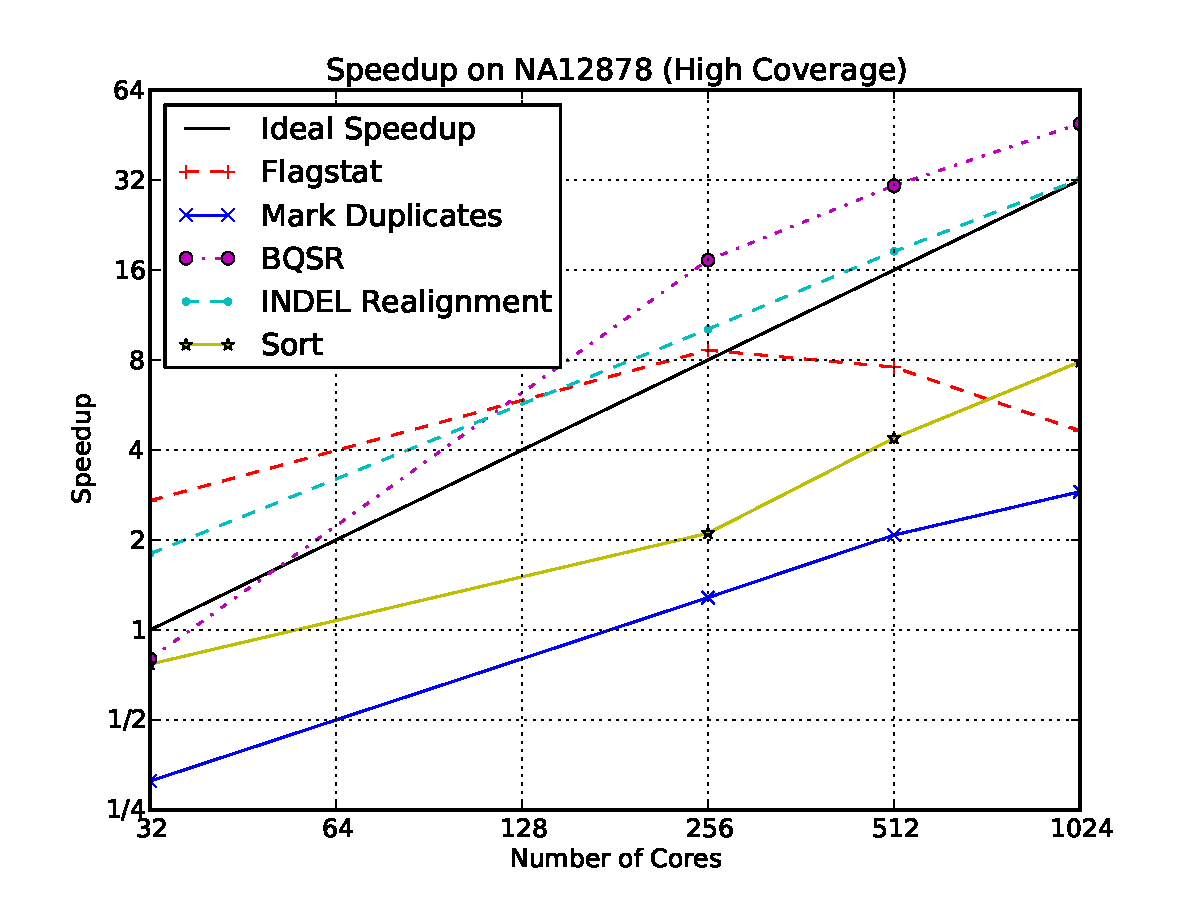
\includegraphics[width=0.99\linewidth]{graphs/speedup_na12878.pdf}
\end{center}
\caption{Speedup on NA12878}
\label{fig:speedup}
\end{figure}

When testing on NA12878, we achieve linear speedup out through 1024 cores; this represents 128
\texttt{m2.4xlarge} nodes. In this test, our performance is limited by several factors:

\begin{itemize}
\item Although columnar stores have very high read performance, they are limited by write performance. Our
tests exaggerate this penalty---as a variant calling pipeline will consume a large read file, but then output a
variant call file that is approximately two orders of magnitude smaller, the write penalty will be reduced. In
practice, we also use in-memory caching to amortize write time across several stages.
\item Additionally, for large clusters, straggler elimination is an issue. However, we have made optimizations to
both the \texttt{Mark Duplicates} and \texttt{INDEL Realignment} code to eliminate stragglers by randomly
rebalancing reads that are unmapped/do not map to a target across partitions.
\end{itemize}

We do note that the performance of \texttt{flagstat} degrades going from 32 to 128 \texttt{m2.4xlarge} nodes.
It is worth noting that \texttt{flagstat} executes in one minute on 32 nodes. By increasing the number of machines
we use to execute this query, we increase scheduling overhead, which leads to degraded performance. While we
have tested against the SAMtools/Picard/GATK pipeline, we do note that new implementations have come out
recently~(e.g., SAMBAMBA and SAMBLASTER~\cite{faust14}) that focus on fast duplicate marking. We have not
compared to them due to time limitations, but will compare to them in a later revision of this paper.

\subsection{Astronomy Workloads}
\label{sec:astro-workloads}

We use the 2MASS data and the Montage test case of 3x3 degree mosaicing with Galaxy m101 as the
center. The tile mosaicing phase has 1.5~GB input data and produces a 1.2~GB aggregated output file.
We compare the \texttt{Spark-mAdd} performance against the High Performance Computing~(HPC)
styled MPI based parallel implementation in Montage v3.3 (\texttt{MPI-mAdd}). We performed the test on
1, 4, and 16 Amazon \texttt{c3.8xlarge} instances. We chose these instances because they provided
HPC-optimized networking, which is necessary for good MPI performance. We use OrangeFS
v2.8.8, a successor of PVFS~\cite{PVFS}, as the shared file system when running \texttt{MPI-mAdd}. All
32 cores on each instance are used for both \texttt{Spark-mAdd} and \texttt{MPI-mAdd}.

\begin{figure}[h]
\begin{center}
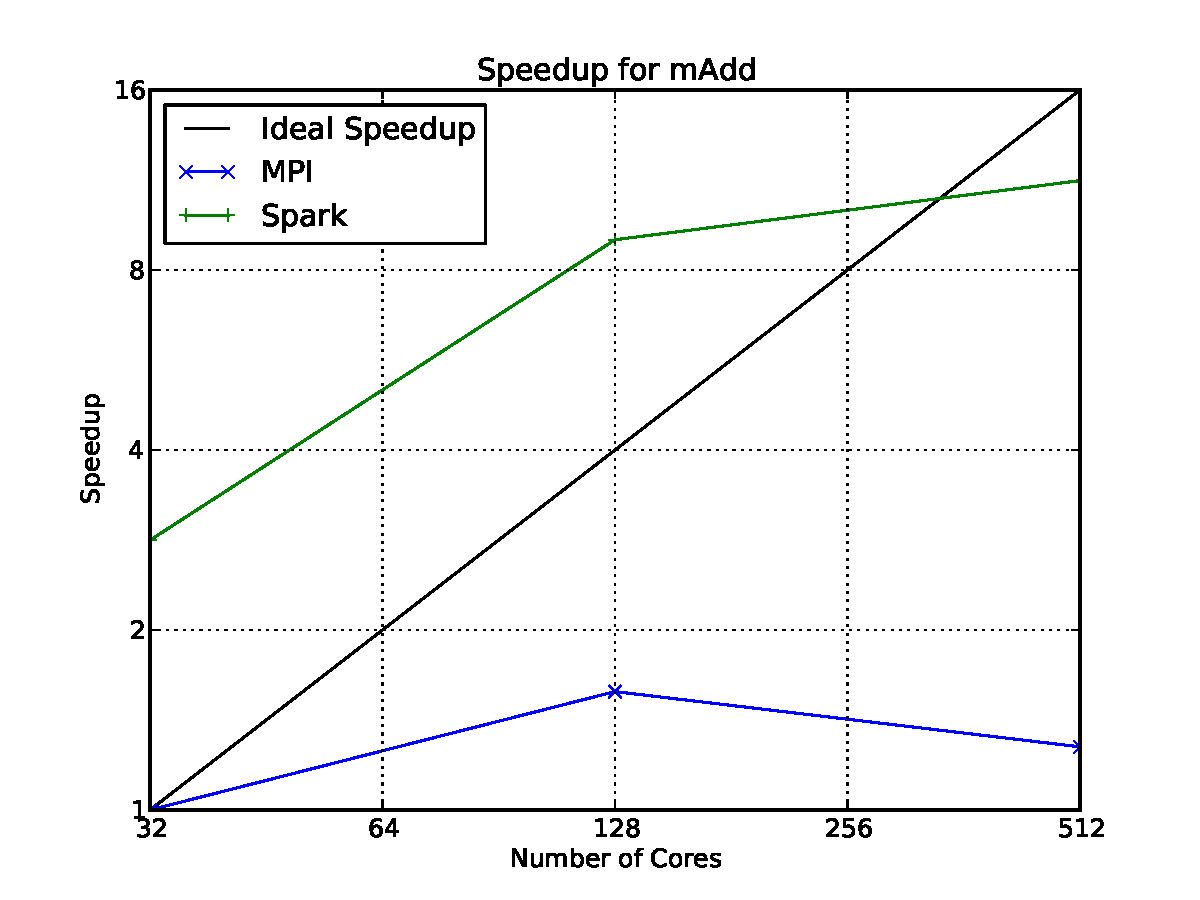
\includegraphics[width=0.99\linewidth]{graphs/speedup_madd.pdf}
\end{center}
\caption{Speedup when running \textit{mAdd} using MPI and Spark}
\label{fig:madd-speedup}
\end{figure}

As shown in Figure~\ref{fig:madd-speedup}, \texttt{Spark-mAdd} runs 2.8x, 5.7x, 8.9x faster than
MPImAdd on 1, 4, and 16 instances with a data compression rate of 2.8x for input and 1.4x for output.
The performance improvement is contributed by multiple factors: less I/O amount, less I/O contention,
and better data locality. We manage to combine the metadata processing stage with mAdd together,
since we explicitly define the data schema in \texttt{Spark-mAdd}, so that the same set of inputs can just
be read once. We also configure Parquet to compress the input and output data, so the actual I/O
amount is reduced. Parquet writes output files into HDFS in a contention free manner whereas MPI
coordinates all processes to write to a single file in the shared file system. The Spark framework lets the
computation benefit from data locality, while MPI distributes the computation across the available
resources without concerning data placement.

\subsection{Column Store Performance}
\label{sec:column-store-perf}

\textbf{FIXME: This uses old data and also needs to be anonymized. Frank to fix. Also, discuss CRAM, and columnar representations for in-memory data.}

The decision to use a columnar store was based on the observation that most genomics applications are read-heavy. In this section,
we aim to quantify the improvements in read performance that we achieve by using a column store, and how far these gains can be
maximized through the use of projections.

\paragraph{Read Length and Quality:}
\label{sec:read-length-and-quality}

This microbenchmark scans all the reads in the file, and collects statistics about the length of the read, and the mapping quality score. Figure~\ref{fig:length-quality} shows
the results of this benchmark. Ideal speedup curves are plotted along with the speedup measurements. The speedups in this graph are plotted relative to the single machine Hadoop-BAM run.

\begin{figure}[h]
\begin{center}
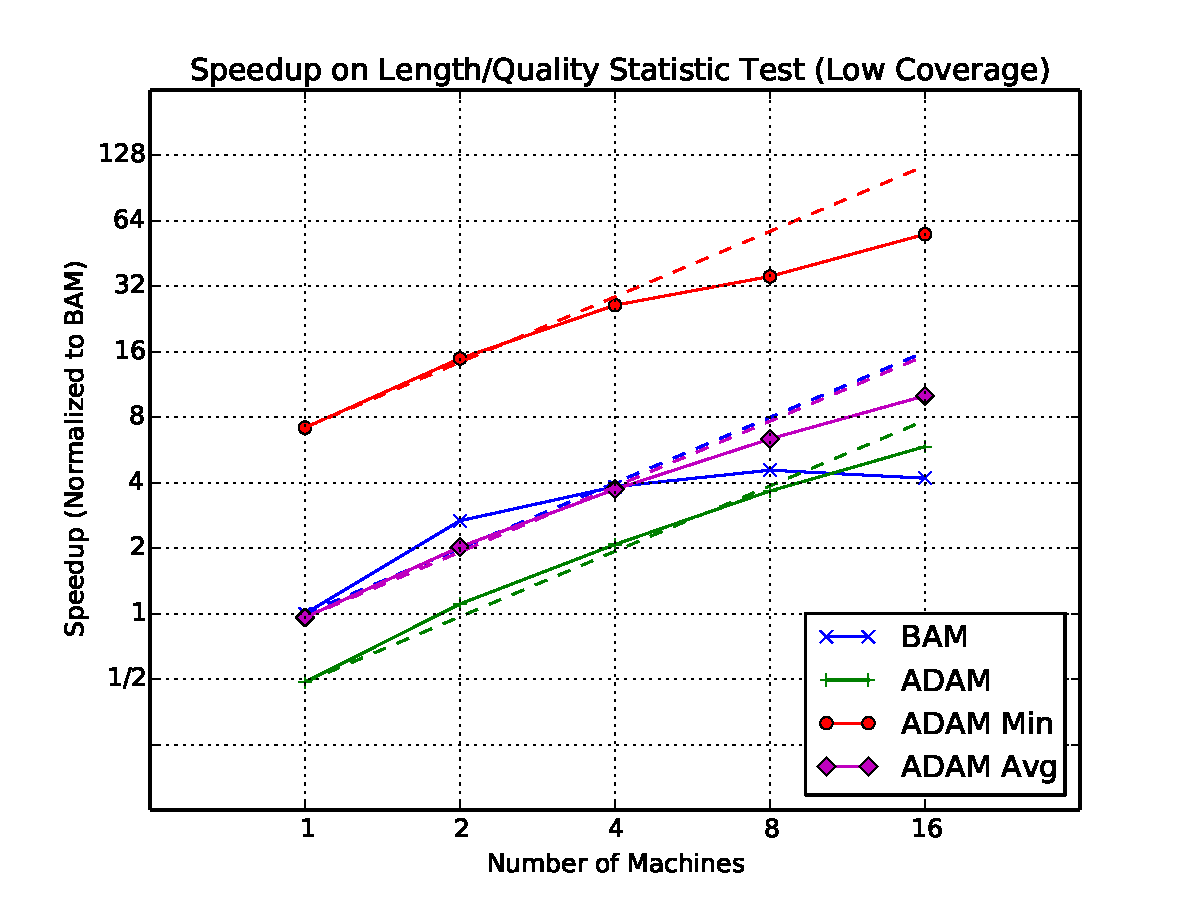
\includegraphics[width=\linewidth]{microbenchmarks/length_and_quality_low_coverage.pdf}
\end{center}
\caption{Read Length and Quality Speedup for HG00096}
\label{fig:length-quality}
\end{figure}

This benchmark demonstrates several things:

\begin{itemize}
\item ADAM demonstrates superior scalability over Hadoop-BAM. This performance is likely because ADAM files can be more evenly distributed across machines.
Hadoop-BAM must guess the proper partitioning when splitting files~\cite{niemenmaa12}. The Parquet file format that ADAM is based on is partitioned
evenly when it is written\cite{parquet}. This paritioning is critical for small files such as the one used in this test~---~in a 16 machine cluster, there is only 1 GB of
data per node, so imbalances on the order of the Hadoop file split size (128 MB) can lead to 40\% differences in loading between nodes.
\item Projections can significantly accelerate computation, if the calculation does not need all the data. By projecting the minimum dataset necessary
to calculate the target of this benchmark, we can accelerate the benchmark by $8\times$. Even a more modest projection leads to a $2\times$
improvement in performance.
\end{itemize}

\subsubsection{Predicate Pushdown}
\label{sec:predicate-pushdown}

Predicate pushdown is one of the significant advantages afforded to us through the use of Parquet	~\cite{parquet}. In traditional
pipelines, the full record is deserialized from disk, and the filter is implemented as a Map/Reduce processing stage. Parquet provides
us with predicate pushdown: we deserialize only the columns needed to identify whether the record should be fully deserialized. We
then process those fields; if they pass the predicate, we then deserialize the full record.

We can prove that this process requires no additional reads. Intuitively, this is true as the initial columns read would need to be read
if they were to be used in the filter later. However, this can be formalized. We provide a proof for this in Section C of the Appendix.
In this section, we seek to provide an intuition for how predicate pushdown can improve the performance of actual genomics workloads.
We apply predicate pushdown to implement read quality predication, mapping score predication, and predication by chromosome. 

\paragraph{Quality Flags Predicate:}
\label{sec:quality-flags-predicate}

This microbenchmark scans the reads in a file, and filters out reads that do not meet a specified quality threshold. We use the following
quality threshold:

\begin{itemize}
\item The read is mapped.
\item The read is at its primary alignment position.
\item The read did not fail vendor quality checks.
\item The read has not been marked as a duplicate.
\end{itemize}
This threshold is typically applied as one of the first operations in any read processing pipeline.

\paragraph{Gapped Predicate:}
\label{sec:gapped-predicate}

In many applications, the application seeks to look at a region of the genome~(e.g. a single chromosome or gene). We include this
predicate as a proxy: the gapped predicate looks for 1 out of every $n$ reads. This selectivity achieves performance analogous to filtering
on a single gene, but provides an upper bound as we pay a penalty due to our predicate hits being randomly distributed.

To validate the performance of predicate pushdown, we ran the predicates described above on the HG00096 genome on a
single AWS $m2.4xlarge$ instance. The goal of this was to determine the rough overhead of predicate projection.

Figure~\ref{fig:gapped-filter} shows performance for the gapped predicate sweeping $n$.

\begin{figure}[h]
\begin{center}
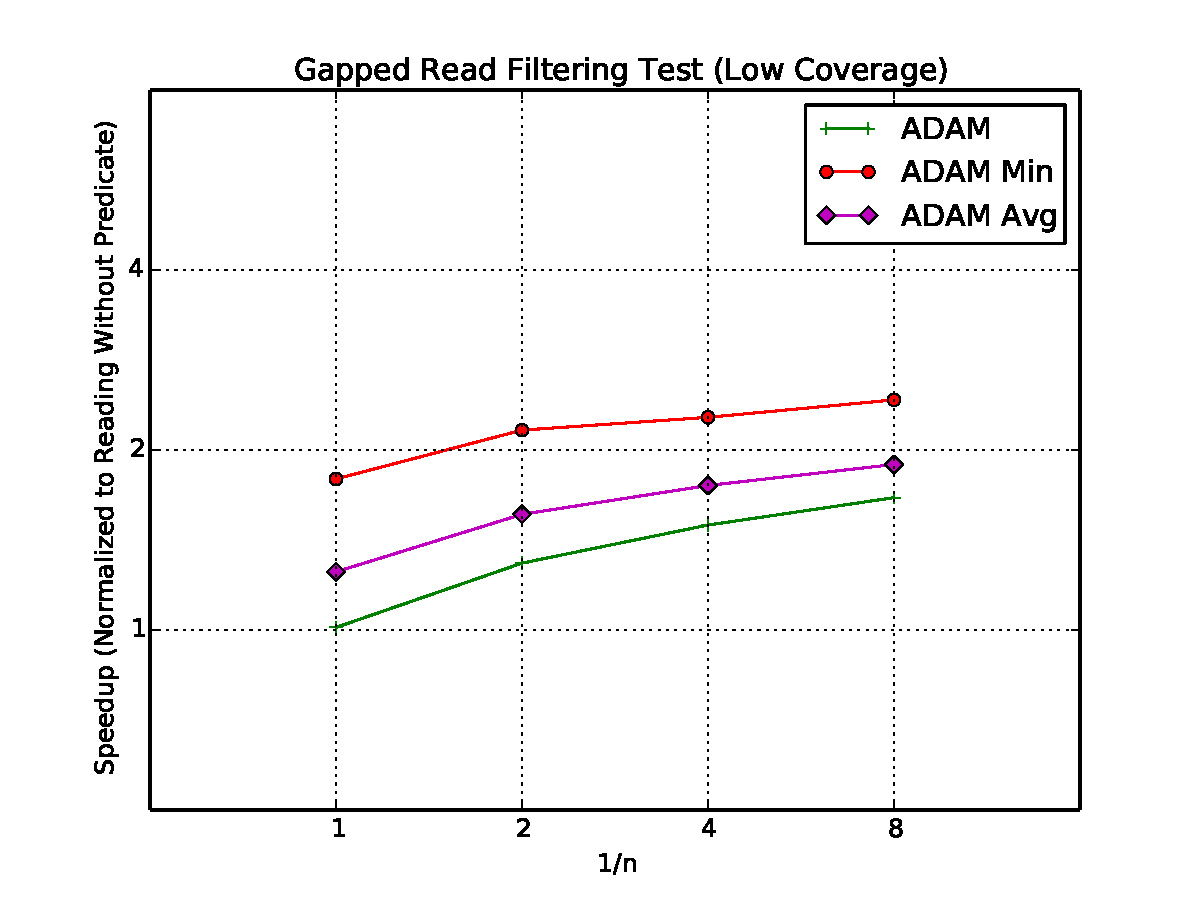
\includegraphics[width=\linewidth]{microbenchmarks/gapped_predicate_low_coverage.pdf}
\end{center}
\caption{Gapped Predicate on HG00096}
\label{fig:gapped-filter}
\end{figure}

There are several conclusions to be drawn from this experiment:

\begin{itemize}
\item As is demonstrated by equation~(\ref{eqn:predicate}) in Section C of the Appendix, we see the largest speedup when our predicate read set is significantly
smaller than our projection read set. For smaller projections, we see a fairly substantial reduction in speedup.
\item As the number of records that passes the predicate drops, the number of reads done to evaluate the predicate begins to become
a dominant term. This insight has one important implication: for applications that plan to access a very small segment of the data, accessing the
data as a flat file with a predicate is likely not the most efficient access pattern. Rather, if the predicate is regular, it is likely better to access
the data through a indexed database.
\end{itemize}

We additionally calculated the performance improvement that was achieved by using predicate pushdown instead of a Spark filter.
Table~\ref{tab:filter-vs-predicate} lists these results.

\begin{table}[h]
\caption{Predicate Pushdown Speedup vs. Filtering}
\label{tab:filter-vs-predicate}
\begin{center}
\begin{tabular}{| l | c  c c | c |}
\hline
\bf Predicate & \bf Min & \bf Avg & \bf Max & \bf Filtered \\
\hline
Locus & 1.19 & 1.17 & 0.94 & 3\% \\
Gapped, $n = 1$ & 1.0 & 1.0 & 1.01 & 0\% \\
Gapped, $n = 2$ & 1.22 & 1.27 & 1.29 & 50\% \\
Gapped, $n = 4$ & 1.31 & 1.42 & 1.49 & 75\% \\
Gapped, $n = 8$ & 1.37 & 1.58 & 1.67 & 87.5\% \\
\hline
\end{tabular}
\end{center}
\end{table}

These results are promising, as they indicate that predicate pushdown is faster than a Spark filter in most cases. We believe that the
only case that showed a slowdown (max projection on Locus predicate) is due to an issue in our test setup. We therefore can conclude
that filtering operations that can be performed statically at file load-in should be performed using predicate pushdown.

\section{Discussion and Future Work}
\label{sec:discussion-future-work}

While we are critical of many scientific systems in~\S\ref{sec:background}, the \texttt{Thunder} system,
which was developed for processing terabytes of neuroscience imaging data~\cite{freeman14} is well
designed. \texttt{Thunder} performs a largely statistical workload, and the significant tasks in terms of
execution time are clustering and regression. The system is constructed using Spark and Python and is
designed to process datasets larger than 4 TB, and leverages significant functionality from the MLI/MLLib
libraries~\cite{sparks13}. Similar to our system, they are able to use Spark's in-memory caching to
amortize load time across several pipeline stages. Additionally, they use Spark's filtering primitives to
allow scientists to cut problems into subproblems. This is a common trend across scientific analyses, and
is one of the reasons that we advocate for the use of a columnar store with efficient predicate pushdown.

This work leverages columnar storage to improve performance and compression of data on disk,
with special emphasis on repetitive fields that can be run length encoded~(RLE). While this improves
disk performance, it has the side effect of making data consume significantly more space in memory
than on disk. We are currently investigating techniques that leverage the immutability of data in our
applications to reduce memory consumption. We have changed Parquet and Avro's deserialization codec
to reuse allocated objects. For every value that is RLE'd, we only allocate the value once in memory. We
then share the value across all records which contained that value. This is especially important since we
maintain a lot of string metadata which is RLE'd on disk.

It is worth noting that there are many significant scientific applications (such as genome
assembly) that are expressed as traversal over graphs. Recent work by Simpson et al~(ABySS,
\cite{simpson09}) and Georganas et al~\cite{georganas14} has focused on using MPI
or Unified Parallel C~(UPC) to implement their own distributed graph traversal. Both systems
find that synchronization via message passing is a significant cost; specifically, the ABySS assembler
experiences scaling problems because it thrashes portions of the graph across nodes during traversal.
By building our system using Spark, we are able to leverage the GraphX processing library~\cite{xin13,
gonzalez14}. We are in the process of developing a genome assembler using this library system, and
believe that we can achieve improved performance through careful graph partitioning. This involves
algorithmic changes to the graph creation and traversal phases to bypass ``knotted'' sections of the
graph that correspond to highly repetitive areas of the genome, which cause the major performance
issues in MPI based assemblers.

\section{Conclusion}
\label{sec:conclusion}

In this paper, we have advocated for a clean architecture for decomposing components in a scientific
system, and then demonstrated how to efficiently implement genomic and astronomy processing
pipelines using the open source Avro, Parquet, and Spark systems~\cite{avro, parquet, zaharia10}.
We demonstrate $22-131\times$ performance improvements over conventional genomics processing
systems, along with linear strong scaling and a $2\times$ cost improvement. On the astronomy
workload, we achieve an average of $5.8\times$ speedup over the current best MPI-based solution at various scales.
Additionally, while
an obvious advantage of using commodity systems is code reuse, we have gained several valuable
features for free:

\begin{enumerate}
\item Beyond efficient parallel performance, Parquet is also supported as a data format by several
database-like systems, like Spark-SQL and Impala. This allows us to support efficient database style
processing, without needing to manually retrofit a tool like GQL to the data~\cite{kozanitis14}.
\item While the native Spark Scala API provides rich programming abstractions, scientists may prefer
other language environments, like Python or R. Other scientific systems like SciDB~\cite{brown10}
support native Python and R bindings. Likewise, we provide distributed processing using Python
through PySpark.
\end{enumerate}

By rethinking the architecture of scientific data management systems, we have been able to achieve
significant scalability improvements while also expanding the methods that can be used to process
the data. The architecture we have developed is clean and principled and minimizes the
mixture-of-concerns that occurs in current scientific systems. Additionally, by applying our techniques
to both astronomy and genomics, we have demonstrated that the techniques are applicable to both
traditional matrix-based scientific computing, as well as novel scientific areas that have less structured
data.

\balancecolumns

\clearpage

\appendix

\bibliographystyle{abbrv}
\bibliography{adam} 

\section{Schemas}
\label{sec:schema}

Here, we present the schemas that we have used for these two systems. We make several
simplifications to the schemas for clarity; specifically, we have grouped all of our fields into a simpler
logical schema ordering, and we have also removed the Avro syntactic sugar used to ensure that all
fields are nullable. These schemas are implemented using Avro~\cite{avro}, and data is stored to disk via
Parquet~\cite{parquet}. In-memory (de-)serialization is provided via a custom wrapper around Avro's
serialization framework.

\subsection{Genomics Schema}
\label{sec:genomics-schema}

The schema used for storing genomics data is described below:

\begin{lstlisting}
record Contig {
  string contigName;
  long contigLength;
  string contigMD5;
  string referenceURL;
  string assembly;
  string species;
}

record AlignmentRecord {
  /** Alignment position and quality */
  Contig contig;
  long start;
  long oldPosition;
  long end;

  /** read ID, sequence, and quality */
  string readName;
  string sequence;
  string qual;
  
  /** alignment details */
  string cigar;
  string oldCigar;
  int mapq;
  int basesTrimmedFromStart;
  int basesTrimmedFromEnd;
  boolean readNegativeStrand;
  boolean mateNegativeStrand;
  boolean primaryAlignment;
  boolean secondaryAlignment;
  boolean supplementaryAlignment;
  string mismatchingPositions;
  string origQual;

  /** Read status flags */
  boolean readPaired;
  boolean properPair;
  boolean readMapped;
  boolean mateMapped;
  boolean firstOfPair;
  boolean secondOfPair;
  boolean failedVendorQualityChecks;
  boolean duplicateRead;

  /** optional attributes */
  string attributes;

  /** record group metadata */
  string recordGroupName;
  string recordGroupSequencingCenter;
  string recordGroupDescription;
  long recordGroupRunDateEpoch;
  string recordGroupFlowOrder;
  string recordGroupKeySequence;
  string recordGroupLibrary;
  int recordGroupPredictedMedianInsertSize;
  string recordGroupPlatform;
  string recordGroupPlatformUnit;
  string recordGroupSample;

  /** Mate pair alignment information */
  long mateAlignmentStart;
  long mateAlignmentEnd;
  Contig mateContig;
}
\end{lstlisting}

All of the metadata from the sequencing run and prior processing steps are packed into the record
group metadata fields. The program information describes the processing lineage of the sample and
is expected to be uniform across all records, thus it compresses extremely well. The record group
information is not guaranteed to be uniform across all records, but there are a limited number number
of record groups per sequencing dataset.\footnote{The record group reflects the way the samples were
sequenced; increasing the parallelism of the sequencing increases the number of record groups.} This
metadata is string heavy, which makes proper deserialization from disk important. Although the
information consumes less than 5\% of space on disk, a poor deserializer implementation may replicate
a string per field per record, which greatly increases the amount of memory allocated and the garbage
collection~(GC) load.

In our system, we have defined common projections and predicates to operate on these records. For
example, tools~(like the \texttt{flagstat} command) that perform quality control for sequenced data
commonly only access the read status flags from the schema. We can reduce the amount of IO we
perform by projecting only these fields. Additionally, it is common to run predicates on the read position,
or whether the read is mapped or not. We have several predicates that are optimized for these queries,
and have devised a system that allows us to apply these predicates to legacy datasets as well; however,
we only get the \emph{functionality} of the predicate, not the performance improvement.

\subsection{Astronomy Schema}
\label{sec:astronomy-schema}

We use the following schema for storing astronomy pixel values:

\begin{lstlisting}
record PixelValue {
  /** pixel position */
  int xPos;
  int yPos;
  
  /** pixel value */
  float value;
  
  /** file metadata */
  int start;
  int end;
  int offset;
  int height;
}
\end{lstlisting}

This schema is derived from the legacy Flexible Image Transport System~(FITS,~\cite{wells81}), which
defines an interchange format for astronomy images. During the \texttt{mAdd} processing kernel
described in~\S{sec:astro-workloads}, we access the file metadata from each pixel. In current systems,
metadata access becomes a significant performance bottleneck as we are performing metadata access
across thousands of files~\cite{zhang13}.

\section{Convex-Hull Finding}
\label{sec:convex-hull}

A frequent pattern in our application is identifying the maximal convex hulls across sets of regions. For
a set $R$ of regions, we define a maximal convex hull as the largest region $\hat{r}$ that satisfies the
following properties:

\begin{align}
\label{eqn:convexity-constraint}
\hat{r} &= \cup_{r_i \in \hat{R}} r_i \\
\hat{r} \cap r_i &\ne \emptyset, \forall r_i \in \hat{R} \\
\hat{R} &\subset R
\end{align}

In our problem, we seek to find all of the maximal convex hulls, given a set of regions. For genomics, the
convexity constraint described by \eqref{eqn:convexity-constraint} is trivial to check: specifically, the
genome is assembled out of reference contigs\footnote{\emph{Contig} is short for \emph{contiguous
sequence}. Reference contigs are normally used to describe the sequence that is unique to each
chromosome.} that define disparate 1-D coordinate spaces. If two regions exist on different contigs, they
are known not to overlap. If two regions are on a single contig, we simply check to see if they overlap
on that contig's 1-D coordinate plane.

Given this realization, we can define the data-parallel algorithm~\ref{alg:parallel-convex-hull} to find the
maximal convex hulls that describe a genomic dataset.

\begin{algorithm}
\caption{Find Convex Hulls in Parallel}
\label{alg:parallel-convex-hull}
\begin{algorithmic}
\STATE $data \leftarrow$ input dataset
\STATE $regions \leftarrow data$.map($data \Rightarrow $generateTarget($data$))
\STATE $regions \leftarrow regions$.sort()
\STATE $hulls \leftarrow regions$.fold($r_1, r_2 \Rightarrow$ mergeTargetSets($r_1, r_2$))
\RETURN $\Theta$
\end{algorithmic}
\end{algorithm}

The \texttt{generateTarget} function projects each datapoint into a Red-Black tree which contains a
single region. The performance of the fold depends on the efficiency of the merge function. We achieve
efficient merges with the tail-call recursive \texttt{mergeTargetSets} function which is described in
algorithm~\ref{alg:join-targets}.

\begin{algorithm}
\caption{Merge Hull Sets}
\label{alg:join-targets}
\begin{algorithmic}
\STATE $first \leftarrow$ first target set to merge
\STATE $second \leftarrow$ second target set to merge
\REQUIRE $first$ and $second$ are sorted
\IF{$first = \emptyset \wedge second = \emptyset$}
\RETURN $\emptyset$
\ELSIF{$first = \emptyset$}
\RETURN $second$
\ELSIF{$second = \emptyset$}
\RETURN $first$
\ELSE
\IF{last($first$) $\cap$ head($second$) $= \emptyset$}
\RETURN $first$ + $second$
\ELSE
\STATE $mergeItem \leftarrow$ (last($first$) $\cup$ head($second$))
\STATE $mergeSet \leftarrow$ allButLast($first$) $\cup mergeItem$
\STATE $trimSecond \leftarrow$ allButFirst($second$)
\RETURN mergeTargetSets($mergeSet$, $trimSecond$)
\ENDIF
\ENDIF
\end{algorithmic}
\end{algorithm}

For a region join~(see~\S\ref{sec:coordinate-system-joins}), we would use the maximal convex hull
set to define partitioning for the join. Alternatively, for INDEL
realignment~(see~\S\ref{sec:local-realignment}), we use this set as an index for mapping reads directly
to targets.

\balancecolumns

\end{document}
